\documentclass{article}
\usepackage[utf8]{inputenc}
\usepackage[brazil]{babel} %hifenização em português do brasil
\usepackage{indentfirst}
\usepackage{amssymb} % caracteres especiais matemáticos 
\usepackage{amsmath}
\usepackage{amsthm}
\usepackage{amsfonts}
\usepackage[pdftex]{graphicx} % figuras
\usepackage{hyperref} %inserir links url

\title{EP02 - Métodos de Monte Carlos\\
MAP2212 - Laboratório de Comutação e Simulação}
\author{Danilo Brito da Silva - Nº USP: 10693250}
\date{19 de abril de 2022}

\begin{document}

\maketitle

\section{Introdução}


Este exercício tem por objetivo estimar a integral de $f(x)$, $x \in [0.1]$ utilizando quatro variantes do Método de Monte Carlo (MMC): \textit{Crud}, \textit{Hit or Miss}, \textit{Importance Sampling} e \textit{Control Variate}.
\begin{equation}
    f(x) = e^{-a x}\cos{bx}
\end{equation}


Utilizaremos $a=0.442705074$ e $b=0.10693250$. Para cada método, o erro relativo deverá ser $\mid\hat{g} - g\mid/g \leq 0.0005$, onde $\hat{g}$ é a estimativa numérica do valor da integral, e $g$ é o verdadeiro valor da integral (desconhecido). \\
Como $g$ é desconhecido, nos apoiaremos no Teorema do Limite Central para estimar o erro, em que, para grandes
números, $\sigma^2 \approx s^2$:
\begin{equation}
    \epsilon = \sqrt{\dfrac{s^2}{n}}
\end{equation}


Para cada um dos métodos, vamos gerar $n$ variáveis pseudo-aleatórias e armazená-las como vetor, calcular variância e erro padrão. Caso o erro seja maior que $0.0005$, aumentamos o $n$ em $2$ vezes e repetimos o processo. O valor da função $g = \int_{0}^{1}f(x)dx$ será estimado como a média dos valores gerados em cada método.

\section{Método Crud}


O valor da integral é calculado como sendo a média dos valores da $f(x)$ em $n$ pontos aleatórios com $x_i$ pertencente ao intervalo $[0, 1]$ e distribuição uniforme, $i=1,...,n$. Portanto, temos:
$$
\hat{g}=\frac{1}{n}\sum_{1}^{n}f(x_i)
$$
Utilizando o Python, rodamos o seguinte código:

Dessa forma, obtivemos os seguintes resutados:\\
$\hat{g}=0.79304; n = 54000;    \epsilon = 0.0005$

\section{Método Hit or Miss}

Neste método, geramos pares de pontos $(x_i,y_i)$ e escolhemos uma função auxiliar $h(x,y)$ de distribuição Bernoulli tal que 
\[
  h(x,y)= \left\{
    \begin{tabular}[]{cc}
     1 & \text{ se } $f(x) \geq y$,\\
     0 & \text{ se } $f(x) < y$.
    \end{tabular}
    \right.
  \]
  
  
  Assim, vamos estimar $g=\int_{0}^{1}\int_{0}^{1}h(x,y)dxdy$ como $\hat{g}=\frac{1}{n}\sum_{1}^{n}h(x_i,y_i)=\frac{n*}{n}$ e a estimativa da variância será dada por $s^2 = \dfrac{\hat{g}(1-\hat{g})}{n}$.
  
  
  Executamos o código abaixo no R e obtivemos os seguintes resultados:\\
 
  $\hat{g}=0.79393; n = 656000;    \epsilon = 0.0005$

\section{Método Importance Sampling}


Neste método, escolhemos uma função auxiliar $k(x)$ que seja função de distribuição de probabilidade conhecida e se aproxime da $f(x)$.

$$
g = \int f(x)dx = \int\frac{f(x)}{k(x)} k(x)dx = \int \frac{f(x)}{k(x)}dK(x)
$$
$$
\hat{g} = \frac{1}{n}\sum_{1}^{n}\frac{f(x_i)}{k(x_i)}, x_i \sim k, i =1:n,s^2 = \frac{1}{n}\int\left(\frac{f(x)}{k(x)} - \hat{g}\right)^2dK(x)
$$


Vamos escolher a função de distribuição Beta($\alpha,\beta$), integrável, razoavelmente proporcional a $f(x)$ e cuja razão $f/Beta$ seja limitada no intervalo $[0,1]$, com $\alpha = 0.9$ e $\beta=1.1$ , ilustrada no gráfico abaixo, e armazenar os resultados de $f(x_i)/k(x_i)$ em um vetor e calcular sua média para chegar na aproximação $\hat{g}$.
\begin{center}
  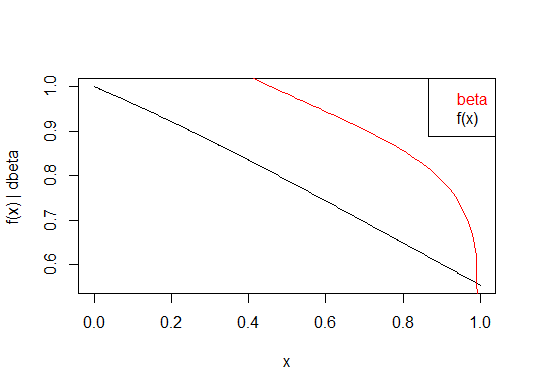
\includegraphics[scale=.55]{./Figuras/plot_beta}\\
\end{center}  



Executando os comandos acima no R, obtivemos os seguintes resultados:\\
 $\hat{g}=0.78075; n = 17000;    \epsilon = 0.00025$

\section{Método Control Variate}


No método Control Variate, escolhemos uma função $\varphi(x)$ de comportamento parecido com a $f(x)$, porém mais fácil de integrar.
$$
g = \int \varphi(x)dx + \int( f(x) - \varphi(x))dx  = g' + \int( f(x) - \varphi(x))dx
$$
Com os estimadores $\hat{g} = \frac{1}{n}\sum_{1}^{n}f(x_i)$ e $\hat{g'} = \frac{1}{n}\sum_{1}^{n}f(x_i)$ e a variância dada por $Var(\hat{g} - \hat{g'}) = Var(\hat{g})+Var(\hat{g'})-2Cov(\hat{g}, \hat{g'})$, o método é útil se as funções $f(x)$ e $\varphi(x)$ possuem forte correlação positiva.


Assim sendo, escolhemos a $\varphi(x) = 1 - 0.5x$, conforme imagem a seguir:

 


No R, armazenamos os valores de $f(x)$ e $\varphi(x)$ e suas diferenças em vetores. Assim, estimamos a integral de $f(x)$ como sendo a média de $\varphi(x)$  mais a média da diferença de $f(x)$ e $\varphi(x)$, conforme abaixo:



Neste método, obtivemos os seguintes resultados:
 $\hat{g}=0.79439; n = 15000;    \epsilon = 0.00049$

\section{Conclusões} 
 
 
O comparativo abaixo nos mostra que os métodos e \textit{Control Variate} e \textit{Importance Sampling} tiveram melhor desempenho do quesito n e erro:

\begin{center}
\begin{tabular}{ |c|c|c|c| } 
 \hline
 Método                       & Estimativa & $n$  & Erro \\ 
 \hline
 \textit{Crud}                & 0.79304 & 54000  & 0.0005 \\ 
 \textit{Hit or Miss}         & 0.79393  & 656000 & 0.0005 \\ 
 \textit{Importance Sampling} & 0.78075  & 17000  & 0.00025 \\ 
 \textit{Control Variate}     & 0.79439  & 15000  & 0.00049 \\ 
 \hline
\end{tabular}
\end{center}

Percebemos que as quatro estimativas são bem próximas umas das outras, com média aritmética de 0.81121245, que nos dá uma boa aproximação do verdadeiro valor de $g$.

Vale destacar que, embora o método \textit{Importance Sampling} tenha dado uma ótima aproximação, ele é muito sensível à escolha da função auxiliar, que poderia nos trazer um resultado mais distante da realidade quando não bem escolhida.




\end{document}